\bta{匀速圆周运动}

\begin{enumerate}[leftmargin=0em]
\renewcommand{\labelenumi}{\arabic{enumi}.}
% A(\Alph) a(\alph) I(\Roman) i(\roman) 1(\arabic)
%设定全局标号series=example	%引用全局变量resume=example
%[topsep=-0.3em,parsep=-0.3em,itemsep=-0.3em,partopsep=-0.3em]
%可使用leftmargin调整列表环境左边的空白长度 [leftmargin=0em]
\item
\exwhere{$ 2019 $年物理江苏卷}
如图所示,摩天轮悬挂的座舱在竖直平面内做匀速圆周运动.座舱的质量为$ m $,运动半径为$ R $,角速度大小为$ \omega $,重力加速度为$ g $,则座舱 \xzanswer{BD} 
\begin{figure}[h!]
\centering
\includesvg[width=0.23\linewidth]{picture/svg/566}
\end{figure}


\fourchoices
{运动周期为$\frac { 2 \pi R } { \omega }$}
{线速度的大小为$ \omega R $}
{受摩天轮作用力的大小始终为$ mg $}
{所受合力的大小始终为$ m \omega ^{2} R $}


\item 
\exwhere{$ 2011 $年理综天津卷}
质量为$ m $的探月航天器在接近月球表面的轨道上飞行,其运动视为匀速圆周运动。已知月球质量为$ M $,月球半径为$ R $,月球表面重力加速度为$ g $,引力常量为$ G $,不考虑月球自转的影响,则航天器的 \xzanswer{AC} 

\fourchoices
{线速度$v = \sqrt { \frac { G M } { R } }$}
{角速度$\omega = \sqrt { g R }$}
{运行周期$T = 2 \pi \sqrt { \frac { R } { g } }$ }
{向心加速度$a = \frac { G m } { R ^ { 2 } }$}

\item 
$ 2013 $年北京卷$ 18 $.某原子电离后其核外只有一个电子,若该电子在核的静电力作用下绕核做匀速圆周运动,那么电子运动 \xzanswer{C} 

\fourchoices
{半径越大,加速度越大}
{半径越小,周期越大}
{半径越大,角速度越小}
{半径越小,线速度越小}



\item 
\exwhere{$ 2014 $年物理上海卷}
如图,带有一白点的黑色圆盘,可绕过其中心、垂直于盘面的轴匀速转动,每秒沿顺时针方向旋转$ 30 $圈。在暗室中用每秒闪光$ 31 $次的频闪光源照射圆盘,观察到白点每秒沿 \xzanswer{D} 
\begin{figure}[h!]
\centering
\includesvg[width=0.14\linewidth]{picture/svg/567}
\end{figure}

\fourchoices
{顺时针旋转$ 31 $圈 }
{逆时针旋转$ 31 $圈}
{顺时针旋转$ 1 $圈 }
{逆时针旋转$ 1 $圈}







\item 
\exwhere{$ 2014 $年理综新课标\lmd{2}卷}
如图,一质量为$ M $的光滑大圆环,用一细轻杆固定在竖直平面内;套在大圆环上的质量为$ m $的小环(可视为质点),从大圆环的最高处由静止滑下,重力加速度为$ g $。当小圆环滑到大圆环的最低点时,大圆环对轻杆拉力的大小为 \xzanswer{C} 
\begin{figure}[h!]
\centering
\includesvg[width=0.14\linewidth]{picture/svg/568}
\end{figure}

\fourchoices
{$ Mg-5mg $ }
{$ Mg+mg $}
{$ Mg+5mg $ }
{$ Mg+10mg $}



\item 
\exwhere{$ 2014 $年理综安徽卷}
如图所示,一倾斜的匀质圆盘绕垂直于盘面的固定对称轴以恒定的角速度$ \omega $转动,盘面上离转轴距离$ 2.5m $处有一小物体与圆盘始终保持相对静止。物体与盘面间的动摩擦因数为$ \frac{\sqrt[4]{3}}{2} $(设最大静摩擦力等于滑动摩擦力),盘面与水平面的夹角为$ 30 \degree $,$ g $取$ 10 \ m/s^{2} $。则$ \omega $的最大值是 \xzanswer{C} 

\begin{figure}[h!]
\centering
\includesvg[width=0.23\linewidth]{picture/svg/569}
\end{figure}

\fourchoices
{$ \sqrt{5}\ rad/s $ }
{$ \sqrt{3}\ rad/s $}
{$ 1.0 \ rad/s $ }
{$ 0.5 \ rad/s $}



\item 
\exwhere{$ 2018 $年江苏卷}
火车以$ 60 $ $ m/s $的速率转过一段弯道,某乘客发现放在桌面上的指南针在$ 10 $ $ s $内匀速转过了约$ 10 ^{ \circ } $。在此$ 10 $ $ s $时间内,火车 \xzanswer{AD} 

\fourchoices
{运动路程为$ 600 $ $ m $ }
{加速度为零}
{角速度约为$ 1 $ $ rad/s $ }
{转弯半径约为$ 3.4 $ $ km $}



\item 
\exwhere{$ 2018 $年浙江卷($ 4 $月选考)}
$ A $、$ B $两艘快艇在湖面上做匀速圆周运动(如图),在相同的时间内,它们通过的路程之比是$ 4:3 $,运动方向改变的角度之比是$ 3:2 $,则它们 \xzanswer{A} 
\begin{figure}[h!]
\centering
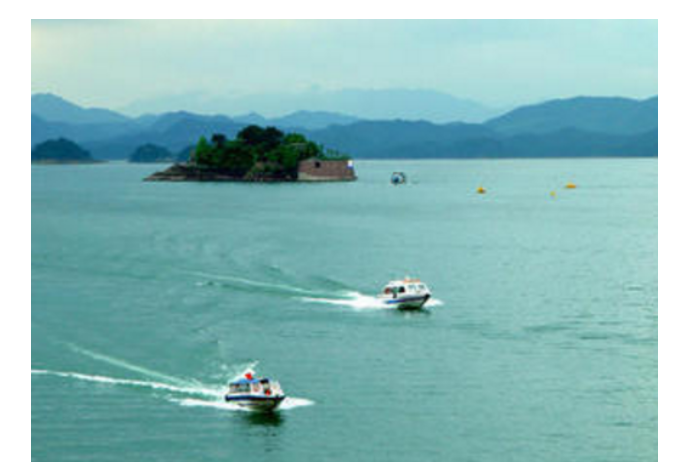
\includegraphics[width=0.3\linewidth]{picture/screenshot004}
\end{figure}

\fourchoices
{线速度大小之比为$ 4:3 $}
{角速度大小之比为$ 3:4 $}
{圆周运动的半径之比为$ 2:1 $}
{向心加速度大小之比为$ 1:2 $}


\newpage	
\item 
\exwhere{$ 2013 $年广东卷}
如图,甲、乙两颗卫星以相同的轨道半径分别绕质量为$ M $和$ 2M $的行星做匀速圆周运动,下列说法正确的是 \xzanswer{A} 

\begin{minipage}[h!]{0.7\linewidth}
\vspace{0.3em}
\fourchoices
{甲的向心加速度比乙的小}
{甲的运行周期比乙的小}
{甲的角速度比乙的大}
{甲的线速度比乙的大}
\vspace{0.3em}
\end{minipage}
\hfill
\begin{minipage}[h!]{0.3\linewidth}
\flushright
\vspace{0.3em}
\includesvg[width=0.8\linewidth]{picture/svg/570}
\vspace{0.3em}
\end{minipage}


\item 
\exwhere{$ 2012 $年理综广东卷}
下图是滑道压力测试的示意图,光滑圆弧轨道与光滑斜面相切,滑道底部$ B $处安装一个压力传感器,其示数$ N $表示该处所受压力的大小,某滑块从斜面上不同高度$ h $处由静止下滑,通过$ B $时,下列表述正确的有 \xzanswer{BC} 
\begin{figure}[h!]
\centering
\includesvg[width=0.36\linewidth]{picture/svg/571}
\end{figure}

\fourchoices
{$ N $小于滑块重力}
{$ N $大于滑块重力}
{$ N $越大表明$ h $越大}
{$ N $越大表明$ h $越小}



\item 
\exwhere{$ 2013 $年新课标 \lmd{2} 卷}
公路急转弯处通常是交通事故多发地带。如图,某公路急转弯处是一圆弧,当汽车行驶的速率为$ vc $时,汽车恰好没有向公路内外两侧滑动的趋势。则在该弯道处 \xzanswer{AC} 
\begin{figure}[h!]
\centering
\includesvg[width=0.23\linewidth]{picture/svg/572}
\end{figure}

\fourchoices
{路面外侧高内侧低}
{车速只要低于$ vc $,车辆便会向内侧滑动}
{车速虽然高于$ vc $,但只要不超出某一最高限度,车辆便不会向外侧滑动}
{当路面结冰时,与未结冰时相比,$ vc $的值变小}



\item 
\exwhere{$ 2013 $年江苏卷}
如图所示,“旋转秋千”中的两个座椅$ A $、$ B $ 质量相等,通过相同长度的缆绳悬挂在旋转圆盘上. 不考虑空气阻力的影响,当旋转圆盘绕竖直的中心轴匀速转动时,下列说法正确的是 \xzanswer{D} 






\begin{minipage}[h!]{0.7\linewidth}
\vspace{0.3em}
\fourchoices
{$ A $ 的速度比$ B $ 的大}
{$ A $ 与$ B $ 的向心加速度大小相等}
{悬挂$ A $、$ B $ 的缆绳与竖直方向的夹角相等}
{悬挂$ A $ 的缆绳所受的拉力比悬挂$ B $ 的小}
\vspace{0.3em}
\end{minipage}
\hfill
\begin{minipage}[h!]{0.3\linewidth}
\flushright
\vspace{0.3em}
\includesvg[width=0.7\linewidth]{picture/svg/573}
\vspace{0.3em}
\end{minipage}



\item 
\exwhere{$ 2015 $年理综福建卷}
如图,在竖直平面内,滑道$ ABC $关于$ B $点对称,且$ A $、$ B $、$ C $三点在同一水平线上。若小滑块第一次由$ A $滑到$ C $,所用时间为$ t_{1} $,第二次由$ C $滑到$ A $,所用时间为$ t_{2} $,小滑块两次的初速度大小相同且运动过程始终沿着滑道滑行,小滑块与滑道的动摩擦因数恒定,则 \xzanswer{A} 
\begin{figure}[h!]
\centering
\includesvg[width=0.23\linewidth]{picture/svg/575}
\end{figure}

\fourchoices
{$ t_{1} < t_{2} $ }
{$ t_{1} = t_{2} $}
{$ t_{1} > t_{2} $ }
{无法比较$ t_{1} $、$ t_{2} $的大小}


\item 
\exwhere{$ 2015 $年理综天津卷}
未来的星际航行中,宇航员长期处于零重力状态,为缓解这种状态带来的不适,有人设想在未来的航天器上加装一段圆柱形“旋转舱”,如图所示,当旋转舱绕其轴线匀速旋转时,宇航员站在旋转舱内圆柱形侧壁上,可以受到与他站在地球表面时相同大小的支持力,为达到上述目的,下列说法正确的是 \xzanswer{B} 
\begin{figure}[h!]
\centering
\includesvg[width=0.23\linewidth]{picture/svg/576}
\end{figure}

\fourchoices
{旋转舱的半径越大,转动的角速度就应越大}
{旋转舱的半径越大,转动的角速度就应越小}
{宇航员质量越大,旋转舱的角速度就应越大}
{宇航员质量越大,旋转舱的角速度就应越小}


\item 
\exwhere{$ 2014 $年理综新课标 \lmd{1}卷}
如图所示,两个质量均为$ m $的小木块$ a $和$ b $(可视为质点)放在水平圆盘上,$ a $与转轴$ OO $′的距离为$ l $,$ b $与转轴的距离为$ 2l $.木块与圆盘的最大静摩擦力为木块所受重力的$ k $倍,重力加速度大小为$ g $,若圆盘从静止开始绕转轴缓慢地加速转动,用$ \omega $表示圆盘转动的角速度.下列说法正确的是 \xzanswer{AC} 
\begin{figure}[h!]
\centering
\includesvg[width=0.23\linewidth]{picture/svg/577}
\end{figure}

\fourchoices
{$ b $一定比$ a $先开始滑动}
{$ a $、$ b $所受的摩擦力始终相等}
{$\omega = \sqrt { \frac { k g } { 2 l } }$是$ b $开始滑动的临界角速度}
{当$\omega = \sqrt { \frac { 2 k g } { 3 l } }$时,$ a $所受摩擦力的大小为$ kmg $}



\newpage	
\item 
\exwhere{$ 2013 $年重庆卷}
如图所示,半径为$ R $的半球形陶罐,固定在可以绕竖直轴旋转的水平转台上,转台转轴与过陶罐球心$ O $的对称轴$ OO ^{\prime} $ 重合。转台以一定角速度$ \omega $匀速转动。一质量为$ m $的小物块落入陶罐内,经过一段时间后,小物块随陶罐一起转动且相对罐壁静止,它和$ O $点的连线与$ OO ^{\prime} $ 之间的夹角$ \theta $为$ 60 ^{ \circ } $。重力加速度大小为$ g $。
\begin{enumerate}
\renewcommand{\labelenumi}{\arabic{enumi}.}
% A(\Alph) a(\alph) I(\Roman) i(\roman) 1(\arabic)
%设定全局标号series=example	%引用全局变量resume=example
%[topsep=-0.3em,parsep=-0.3em,itemsep=-0.3em,partopsep=-0.3em]
%可使用leftmargin调整列表环境左边的空白长度 [leftmargin=0em]
\item
若$ \omega = \omega _0 $,小物块受到的摩擦力恰好为零,求$ \omega_ 0 $;
\item 
$ \omega =(1 \pm k) \omega_ 0 $,且$ 0 <k <<1 $,求小物块受到的摩擦力大小和方向。



\end{enumerate}
\begin{figure}[h!]
\flushright
\includesvg[width=0.29\linewidth]{picture/svg/578}
\end{figure}

\banswer{
\begin{enumerate}
\renewcommand{\labelenumi}{\arabic{enumi}.}
% A(\Alph) a(\alph) I(\Roman) i(\roman) 1(\arabic)
%设定全局标号series=example	%引用全局变量resume=example
%[topsep=-0.3em,parsep=-0.3em,itemsep=-0.3em,partopsep=-0.3em]
%可使用leftmargin调整列表环境左边的空白长度 [leftmargin=0em]
\item
$\omega _ { 0 } = \sqrt { 2 g / R }$
\item 
静摩擦力沿切线向下,$f = \frac { \sqrt { 3 } k ( 2 + k ) } { 2 } m g$


\end{enumerate}


}







\item 
\exwhere{$ 2015 $年理综山东卷}
如图甲所示,物块与质量为$ m $的小球通过不可伸长的轻质细绳跨过两等高定滑轮连接。物块置于左侧滑轮正下方的表面水平的压力传感装置上,小球与右侧滑轮的距离为$ l $. 开始时物块和小球均静止,将此时传感装置的示数记为初始值。现给小球施加一始终垂直于$ l $段细绳的力,将小球缓慢拉起至细绳与竖直方向成$ 60 ^{ \circ } $角,如图乙所示,此时传感装置的示数为初始值的$ 1.25 $倍;再将小球由静止释放,当运动至最低位置时,传感装置的示数为初始值的$ 0.6 $倍。不计滑轮的大小和摩擦,重力加速度的大小为$ g $。求:
\begin{enumerate}
\renewcommand{\labelenumi}{\arabic{enumi}.}
% A(\Alph) a(\alph) I(\Roman) i(\roman) 1(\arabic)
%设定全局标号series=example	%引用全局变量resume=example
%[topsep=-0.3em,parsep=-0.3em,itemsep=-0.3em,partopsep=-0.3em]
%可使用leftmargin调整列表环境左边的空白长度 [leftmargin=0em]
\item
物块的质量;
\item 
从释放到运动至最低位置的过程中,小球克服空气阻力所做的功。 


\end{enumerate}
\begin{figure}[h!]
\flushright
\includesvg[width=0.43\linewidth]{picture/svg/580}
\end{figure}


\banswer{
\begin{enumerate}
\renewcommand{\labelenumi}{\arabic{enumi}.}
% A(\Alph) a(\alph) I(\Roman) i(\roman) 1(\arabic)
%设定全局标号series=example	%引用全局变量resume=example
%[topsep=-0.3em,parsep=-0.3em,itemsep=-0.3em,partopsep=-0.3em]
%可使用leftmargin调整列表环境左边的空白长度 [leftmargin=0em]
\item
$ 3m $
\item 
$ 0.1mgl $


\end{enumerate}


}

\newpage

\item 
\exwhere{$ 2015 $年上海卷}
如图,质量为$ m $的小球用轻绳悬挂在$ O $点,在水平恒力$ F=mg \tan \theta $作用下,小球从静止开始由$ A $经$ B $向$ C $运动。则小球 \xzanswer{ACD} 




\begin{minipage}[h!]{0.7\linewidth}
\vspace{0.3em}
\fourchoices
{先加速后减速}
{在$ B $点加速度为零}
{在$ C $点速度为零}
{在$ C $点加速度为$ g \tan \theta $}
\vspace{0.3em}
\end{minipage}
\hfill
\begin{minipage}[h!]{0.3\linewidth}
\flushright
\vspace{0.3em}
\includesvg[width=0.5\linewidth]{picture/svg/579}
\vspace{0.3em}
\end{minipage}

\item 
\exwhere{$ 2015 $年理综浙江卷}
如图所示为赛车场的一个水平“$ U $”形弯道,转弯处为圆心在$ O $点的半圆,内外半径分别为$ r $和$ 2r $。一辆质量为$ m $的赛车通过$ AB $线经弯道到达$ A ^{\prime} B ^{\prime} $ 线,有如图所示的①②③三条路线,其中路线③是以$ O ^{\prime} $ 为圆心的半圆,$ OO ^{\prime} =r $。赛车沿圆弧路线行驶时,路面对轮胎的最大径向静摩擦力为$ F_{max} $。选择路线,赛车以不打滑的最大速率通过弯道(所选路线内赛车速率不变,发动机功率足够大),则 \xzanswer{ACD} 
\begin{figure}[h!]
\centering
\includesvg[width=0.23\linewidth]{picture/svg/581}
\end{figure}

\fourchoices
{选择路线①,赛车经过的路程最短}
{选择路线②,赛车的速率最小}
{选择路线③,赛车所用时间最短}
{①②③三条路线的圆弧上,赛车的向心加速度大小相等}


\item 
\exwhere{$ 2016 $年新课标$ \lmd{2} $卷}
小球$ P $和$ Q $用不可伸长的轻绳悬挂在天花板上,$ P $球的质量大于$ Q $球的质量,悬挂$ P $球的绳比悬挂$ Q $ 球的绳短。将两球拉起,使两绳均被水平拉直,如图所示。将两球由静止释放,在各自轨迹的最低点 \xzanswer{C} 
\begin{figure}[h!]
\centering
\includesvg[width=0.23\linewidth]{picture/svg/582}
\end{figure}

\fourchoices
{$ P $球的速度一定大于$ Q $球的速度}
{$ P $球的动能一定小于$ Q $球的动能}
{$ P $球所受绳的拉力一定大于$ Q $球所受绳的拉力}
{$ P $球的向心加速度一定小于$ Q $球的向心加速度}



\item 
\exwhere{$ 2016 $年四川卷}
国务院批复,自$ 2016 $年起将$ 4 $月$ 24 $日设立为“中国航天日”。$ 1970 $年$ 4 $月$ 24 $日我国首次成功发射的人造卫星东方红一号,目前仍然在椭圆轨道上运行,其轨道近地点高度约为$ 440 $ $ km $,远地点高度约为$ 2060 $ $ km $;$ 1984 $年$ 4 $月$ 8 $日成功发射的东方红二号卫星运行在赤道上空$ 35786 $ $ km $的地球同步轨道上。设东方红一号在远地点的加速度为$ a_{1} $,东方红二号的加速度为$ a_{2} $,固定在地球赤道上的物体随地球自转的加速度为$ a_{3} $,则$ a_{1} $、$ a_{2} $、$ a_{3} $的大小关系为 \xzanswer{D} 

\fourchoices
{$ a_{2} > a_{1} >a_{3} $ }
{$ a_{3} >a_{2} > a_{1} $}
{$ a_{3} >a_{1} > a_{2} $ }
{$ a_{1} >a_{2} > a_{3} $}



\item 
\exwhere{$ 2016 $年海南卷}
如图,光滑圆轨道固定在竖直面内,一质量为$ m $的小球沿轨道做完整的圆周运动。已知小球在最低点时对轨道的压力大小为$ N_{1} $,在高点时对轨道的压力大小为$ N_{2} $.重力加速度大小为$ g $,则$ N_{1} $–$ N_{2} $的值为 \xzanswer{D} 


\begin{minipage}[h!]{0.7\linewidth}
\vspace{0.3em}
\fourchoices
{$ 3mg $}
{$ 4mg $}
{$ 5mg $}
{$ 6mg $}
\vspace{0.3em}
\end{minipage}
\hfill
\begin{minipage}[h!]{0.3\linewidth}
\flushright
\vspace{0.3em}
\includesvg[width=0.45\linewidth]{picture/svg/583}
\vspace{0.3em}
\end{minipage}



\item 
\exwhere{$ 2016 $年上海卷}
风速仪结构如图$ (a) $所示。光源发出的光经光纤传输,被探测器接收,当风轮旋转时,通过齿轮带动凸轮圆盘旋转,当圆盘上的凸轮经过透镜系统时光被遮挡。已知风轮叶片转动半径为$ r $,每转动$ n $圈带动凸轮圆盘转动一圈。若某段时间$ \Delta t $内探测器接收到的光强随时间变化关系如图$ (b) $所示,则该时间段内风轮叶片 \xzanswer{B} 
\begin{figure}[h!]
\centering
\includesvg[width=0.43\linewidth]{picture/svg/584}
\end{figure}


\fourchoices
{转速逐渐减小,平均速率为$\frac { 4 \pi n r } { \Delta t }$}
{转速逐渐减小,平均速率为$\frac { 8 \pi n r } { \Delta t }$}
{转速逐渐增大,平均速率为$\frac { 4 \pi n r } { \Delta t }$}
{转速逐渐增大,平均速率为$\frac { 8 \pi n r } { \Delta t }$}





\item 
\exwhere{$ 2016 $年浙江卷}
如图所示为赛车场的一个“梨形”赛道,两个弯道分别为半径$ R=90m $的大圆弧和$ r=40m $的小圆弧,直道与弯道相切。大、小圆弧圆心$ O $、$ O ^{\prime} $ 距离$ L=100m $。赛车沿弯道路线行驶时,路面对轮胎的最大径向静摩擦力是赛车重力的$ 2.25 $倍,假设赛车在直道上做匀变速直线运动,在弯道上做匀速圆周运动,要使赛车不打滑,绕赛道一圈时间最短(发动机功率足够大,重力加速度$ g=10 \ m/s^{2} ,\pi=3.14 $)。 \xzanswer{AB} 
\begin{figure}[h!]
\centering
\includesvg[width=0.21\linewidth]{picture/svg/585}
\end{figure}

\fourchoices
{在绕过小圆弧弯道后加速}
{在大圆弧弯道上的速率为$ 45 $ $ m/s $}
{在直道上的加速度大小为$ 5.63 $ $ m/s^{2} $}
{通过小圆弧弯道的时间为$ 5.85 $ $ s $}


\item 
\exwhere{$ 2016 $年天津卷}
我国即将发射“天宫二号”空间实验室,之后发生“神舟十一号”飞船与“天宫二号”对接。假设“天宫二号”与“神舟十一号”都围绕地球做匀速圆周运动,为了实现飞船与空间实验室的对接,下列措施可行的是 \xzanswer{C} 


\fourchoices
{使飞船与空间实验室在同一轨道上运行,然后飞船加速追上空间实验室实现对接}
{使飞船与空间实验室在同一轨道上运行,然后空间实验室减速等待飞船实现对接}
{飞船先在比空间实验室半径小的轨道上加速,加速后飞船逐渐靠近空间实验室,两者速度接近时实现对接}
{飞船先在比空间实验室半径小的轨道上减速,减速后飞船逐渐靠近空间实验室,两者速度接近时实现对接}





\item 
\exwhere{$ 2017 $年江苏卷}
如图所示,一小物块被夹子夹紧,夹子通过轻绳悬挂在小环上,小环套在水平光滑细杆上,物块质量为$ M $,到小环的距离为$ L $,其两侧面与夹子间的最大静摩擦力均为$ F $,小环和物块以速度$ v $向右匀速运动,小环碰到杆上的钉子$ P $后立刻停止,物块向上摆动,整个过程中,物块在夹子中没有滑动,小环和夹子的质量均不计,重力加速度为$ g $. 下列说法正确的是 \xzanswer{D} 
\begin{figure}[h!]
\centering
\includesvg[width=0.23\linewidth]{picture/svg/586}
\end{figure}

\fourchoices
{物块向右匀速运动时,绳中的张力等于$ 2F $}
{小环碰到钉子$ P $时,绳中的张力大于$ 2F $}
{物块上升的最大高度为$\frac { 2 v ^ { 2 } } { g }$}
{速度$ v $不能超过 $\sqrt { \frac { ( 2 F - M g ) L } { M } }$}









\end{enumerate}

